\section{Modules}
\label{sec:modules}

This section provides an overview of the main modules that are used in
an SRAM.  For each module, we will provide both an architectural
description and an explanation of how that design is generated and
used in OpenRAM.  The modules described below are provided in the
first release of OpenRAM, but by no means is this an exhaustive list
of the possible circuits that can be adapted into a SRAM architecture;
refer to Section~\ref{sec:implementation} for more information on
adding different module designs to the compiler.

Each module has a corresponding python class in the \verb|compiler|
directory.  These classes are used to generate both the GDSII layout
and spice netlists. Each module can consist of library cells as
discussed in Section~\ref{sec:techdir}, paramterized cells in
Section~\ref{sec:parameterized} or other modules.  A discussion of the
design hierarchy and how to implement a module is provided in
Section~\ref{sec:design}.

When combining modules at any level of hierarchy, DRC rules for
minimum spacing of metals, wells, etc. must be followed and DRC and
LVS are run by default after each hierarchical module's creation.


\subsection{The Bitcell and Bitcell Array}
\label{sec:bitcellarray}

The 6T cell is the most commonly used memory cell in SRAM devices.  It
is named a 6T cell because it consist of 6 transistors: 2 access
transistors and 2 cross coupled inverters as shown in
Figure~\ref{fig:6t_cell}.  The cross coupled inverters hold a single
data bit that can either be driven into, or read from the cell by the
bitlines.  The access transistors are used to isolate the cell from
the bitlines so that data is not corrupted while a cell is not being
accessed.

\begin{figure}[h!]
\centering
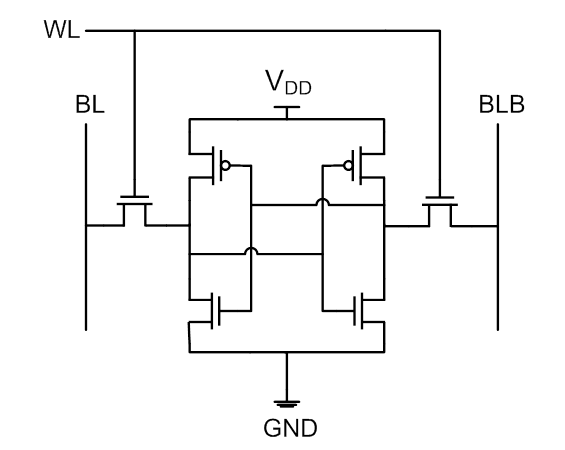
\includegraphics[scale=.9]{./figs/cell_6t_schem.pdf}
\caption{Schematic of 6T cell.}
\label{fig:6t_cell}
\end{figure}

% memory cell operation
The 6T cell can be accessed to perform the two main operation
associated with memory: reading and writing.  When a read is to be
performed, both bitlines are precharged to VDD.  This precharging is
done during the first half of the read cycle and is handled by the
precharge circuitry.  In the second half of the read cycle the
wordline is asserted, which enable the access transistors.  If a 1 is
stored in the cell then BLB is discharged to Gnd and BL is pulled up
to Vdd.  Conversely, if the value stored is a 0, then BL is discharged
to Gnd and BLB is pulled up to Vdd.  While performing a write
operation, both bitlines are also precharged to Vdd during the first
half of the write cycle.  Again, the world line is asserted, and the
access transistors are enabled.  The value that is to be written into
the cell is applied to BL, and its complement is applied to BLB.  The
drivers that are applying the signals to the bitlines must be
appropriately sized so that the previous value in the cell can be
overwritten.

% tiling memory cells
The 6T cells are tiled together in both the horizontal and vertical
directions to make up the memory array.  The size of the memory array
is directly related to the numbers of words, and the size of those
words, that will need to be stored in the RAM.  For example, an 8kb
memory with a word size of 8 bits could be implemented as 8 columns
and 1024 rows.  

% keeping it square
It is common practice to keep the aspect ratio of memory array as
square as possible\footnote{Future versions will consider optimizing
  delay and/or power as well.}.  This helps to make sure that the
bitlines do not become too long, which can increase the bitline
capacitance, slow down the operation and lead to more leakage.  To
make the design ``more square'', multiple words can share rows by
interleaving the bits of each word.  If the previous 8kb memory was
rearranged to allow 2 words per row, then the array would have 16
columns and 512 rows.  

% memory cell is a library cell
In OpenRAM, we provide a library cell for the 6T cell so that users
can easily swap in different memory cell designs.  The memory cell is
the most important cell in the RAM and should be customized to
minimize area and optimize performance.  The memory cell is the most
replicated cell in the RAM; minimizing its size can have a drastic
effext on the overall size of the RAM.  Also, the transitors in the cell
must be carefully sized to allow for correct read and write operation
as well as protection against corruption.

% bitcell and bitcell_array classes
The \verb|bitcell| class in \verb|bitcell.py| instantiates a single
memory cell and is usually a pre-made library cell. The
\verb|bitcell_array| class in \verb|bitcell_array.py| dynamically
implements the memory cell array by instantiating a single memory cell
according to the number of rows and columns.  During the tiling
process, the cells are abutted so that all bitlines and word lines are
connected in the vertical and horizontal directions respectively.  In
order to share supply rails, cells are flipped in alternating rows. To
avoid any extra routing, the power/ground rails, bitlines, and
wordlines should span the entire width/height of the cell so thay they
are automatically connected when the cells are abutted.


\subsection{Precharge Circuitry}
\label{sec:precharge}

The precharge circuit is depicted in Figure~\ref{fig:precharge} and is
implemented by three PMOS transistors. The input signal to the cell,
clk, enables all three transistors during the first half of a read or
write cycle (i.e. while the clock signal is low).  M1 and M2 charge BL
and BLB to Vdd and M3 helps to equalize the voltages seen on BL and
BLB.

\begin{figure}[h!]
\centering
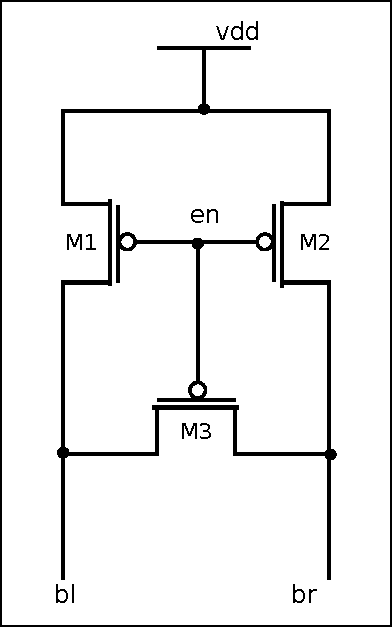
\includegraphics[width=5cm]{./figs/precharge_schem.pdf}
\caption{Schematic of a single precharge cell. \fixme{Change PCLK to CLK.}}
\label{fig:precharge}
\end{figure}

In OpenRAM, the precharge citcuitry is dynamically generated using the
parameterized transistor class (\verb|ptx|). The \verb|precharge|
class in \verb|precharge.py| dynamically generates a single precharge cell.

The offsets of the bitlines and the width of the precharge cell are
equal to the 6T cell so that the bitlines are correctly connected down
to the 6T cell.  The \verb|precharge_array| class is then used to
generate a precharge array, which is a single row of \textbf{n}
precharge cells, where \textbf{n} equals the number of columns in the
bitcell array.


\subsection{Address Decoders}
\label{sec:addressdecoder}

The address decoder takes the row address bits from the address bus as
inputs, and asserts the appropriate wordline in the row that data is
to be read or written.  A n-bit address input controls $2^n$ word
lines. 

OpenRAM provides a hierarchical address decoder as the default, but
will soon have other options.

\subsubsection{Hierarchical Decoder}
\label{sec:hierdecoder}

Hierarchical decoder is a type of decoder which the constrcution takes place hierarchically. 
The simple 2:4 decoder is shown in the Figure~\ref{fig:2 to 4 decoder}. The operation of
this decoder can be explained as follows: soon after the address signals A0 and A1 are put on the address lines, 
depending on the signal combination, one of the wordlines will rise after a brief amount of time. For example if the
address input is A0A1=00 then the output is W0W1W2W3=1000. The 2:4 address decoder uses inverters and two 
input nand gates for its constrcution while the gates are sized to have equal rise and fall time.
As the decoder size increases the size of the nand gates required for decoding also increases.
Table~\ref{table:2-4 hierarchical_decoder} gives the detailed input and output siganls
for the 2:4 hierarchical decoder. 


\begin{figure}[h!]
\centering
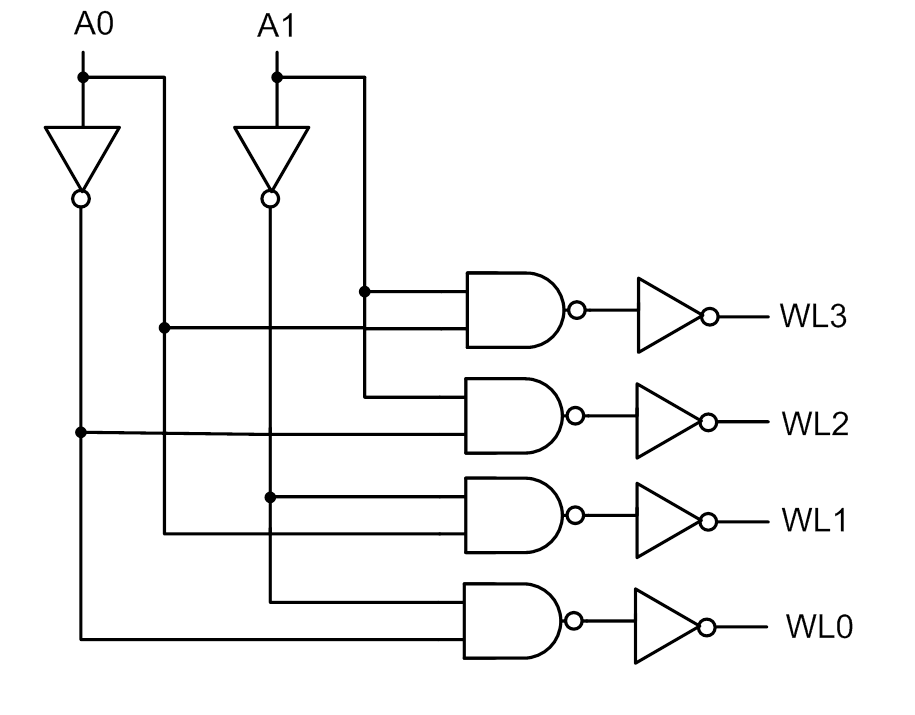
\includegraphics[scale=.6]{./figs/2t4decoder.pdf}
\caption{Schematic of 2-4 simple decoder.}
\label{fig:2 to 4 decoder}
\end{figure}

 \begin{table}[h!] 
   \begin{center}
     \begin{tabular}{| c | c |}
     \hline
     A[1:0] & Selected WL\\ \hline
     00 & 0\\ \hline
     01 & 1\\ \hline
     10 & 2\\ \hline
     11 & 3\\ \hline

     \end{tabular}
   \end{center}
   \caption{Truth table for 2:4 hierarchical decoder.}
   \label{table:2-4 hierarchical_decoder}
 \end{table}


An $n$-bit decoder requires {$2^n$} logic gates, each with $n$ inputs. For example, with $n$ = 6, 
64 $NAND6$ gates are needed to drive 64 inverters to implement the decoder.
It is clear that gates with more than 3 inputs create large series resistances and long delays. 
Rather than using $n$-input gates, it is preferable to use a cascade of gates. 
Typically two stages are used: a predecode stage and a final decode stage. 
The predecode stage generates intermediate signals that are used 
by multiple gates in the final decode stage.



\begin{figure}[h!]
\centering
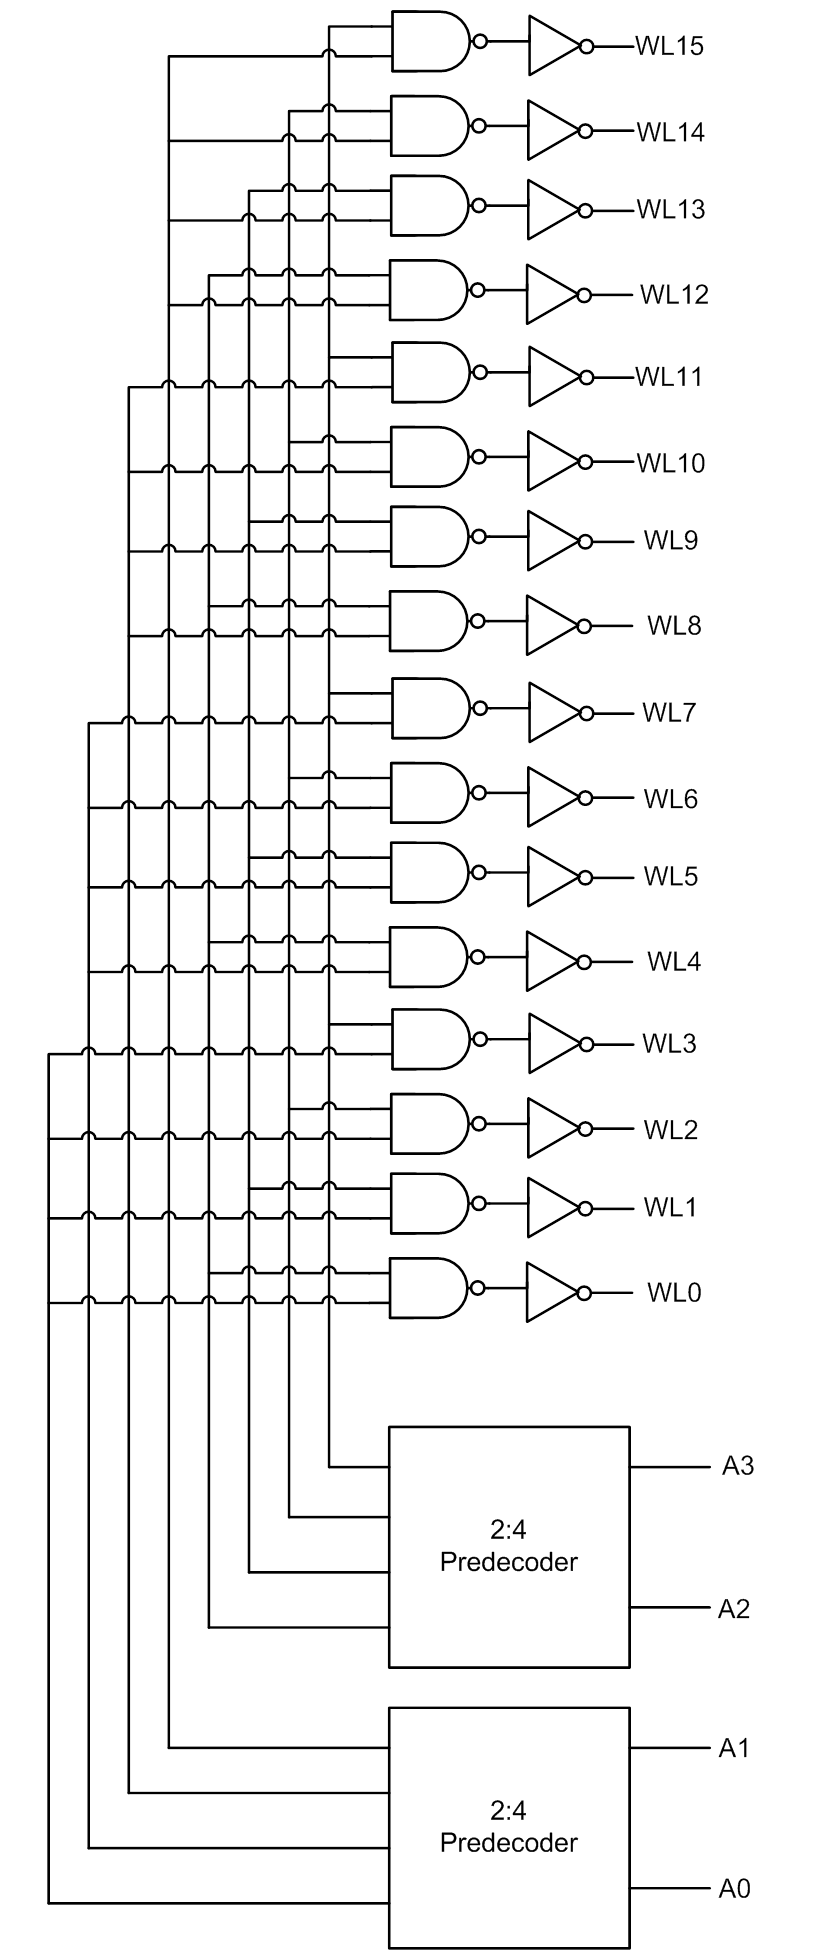
\includegraphics[scale=.6]{./figs/4t16decoder.pdf}
\caption{Schematic of 4 to 16 hierarchical decoder.}
\label{fig:4 to 16 decoder}
\end{figure}

Figure~\ref{fig:4 to 16 decoder} shows the 4 to 16 heirarchical decoder. The structure of the decoder consists of two 2:4 decoders for predecoding and 2-input nand gates and inverters for final decoding to form the 4:16 decoder.
In the predecoder, a total of 8 intermediate signals are generated from the address bits and their complements.
The concept of using predecoing and final decoding stage for construction of address decoder is very procutive since small
decoders like 2:4 decoder is used for predecoding. The operation of 4:16 heirarchical decoder can explained with an example. If the address is A0A1A2A3=0000 the output of the predecoder1 and predeocder2 will be
WL0WL1WL2WL3=1000 and WL0WL1WL2WL3=1000, respectively. According to the connections in figure~\ref{fig:4 to 16 decoder} the wordline 0 of predecoder1 and predecoder2 are conneted 
to the first 2-input nand gate in the decode stage representing the wordline 0 of the final decoding stage. Hence depengin on the combination
of the input signal one of the wordline will rise. In this case since the address input is A0A1A2A3=0000 the wordline 0 should go high. Table~\ref{table:4-16 hierarchical_decoder} gives the detailed input and output siganls
for the 4:16 hierarchical decoder.


 \begin{table}[h!] 
   \begin{center}
     \begin{tabular}{| c | c | c | c |}
     \hline
     A[3:0] & predecoder1 & predecoder2 & Selected WL\\ \hline
     0000 & 1000 & 1000 & 0\\ \hline
     0001 & 1000 & 0100 & 1\\ \hline
     0010 & 1000 & 0010 & 2\\ \hline
     0011 & 1000 & 0001 & 3\\ \hline
     0100 & 0100 & 1000 & 4\\ \hline
     0101 & 0100 & 0100 & 5\\ \hline
     0110 & 0100 & 0010 & 6\\ \hline
     0111 & 0100 & 0001 & 7\\ \hline
     1000 & 0010 & 1000 & 8\\ \hline
     1001 & 0010 & 0100 & 9\\ \hline
     1010 & 0010 & 0010 & 10\\ \hline
     1011 & 0010 & 0001 & 11\\ \hline
     1100 & 0001 & 1000 & 12\\ \hline
     1101 & 0001 & 0100 & 13\\ \hline
     1110 & 0001 & 0010 & 14\\ \hline
     1111 & 0001 & 0001 & 15\\ \hline
     \end{tabular}
   \end{center}
   \caption{Truth table for 4:16 hierarchical decoder.}
   \label{table:4-16 hierarchical_decoder}
 \end{table}


As the size of the address line increases higher level decoder can be created using the lower level decoders. For example for a 8:256 decoder, two instances of 4:16 followed by 256 2-input nand gates and inverters 
can form the decoder. In order to construct the 8:256 decoder, first 4:16 decoder should be constructed through using 2:4 deccoders. Hence the name is hierarchical decoder.


\subsection{Wordline Driver}
\label{sec:wldriver}

Word line drivers are inserted, in between the word line
output of the address decoder and the word line input of the bitcell-array.  The word
line drivers ensure that as the size of the memory array increases,
and the word line length and capacitance increases, the word line
signal is able to turn on the access transistors in the 6T cell. Also, as the bank select signal
in multi-bank structures is $ANDED$ with the word line output of decoder, 
bitcells turn on only when bank is selected. 
Figure~\ref{fig:wordline_driver} shows the diagram of word line driver and its input/output pins.
In OpenRAM, word line drivers are created by using the \verb|pinv| and \verb|nand2| classes which
takes the transistor size and cell height as inputs (so that it can abutt the
6T cell). Word line driver is added as seperate module in \verb|compiler|.
\begin{figure}[h!]
\centering
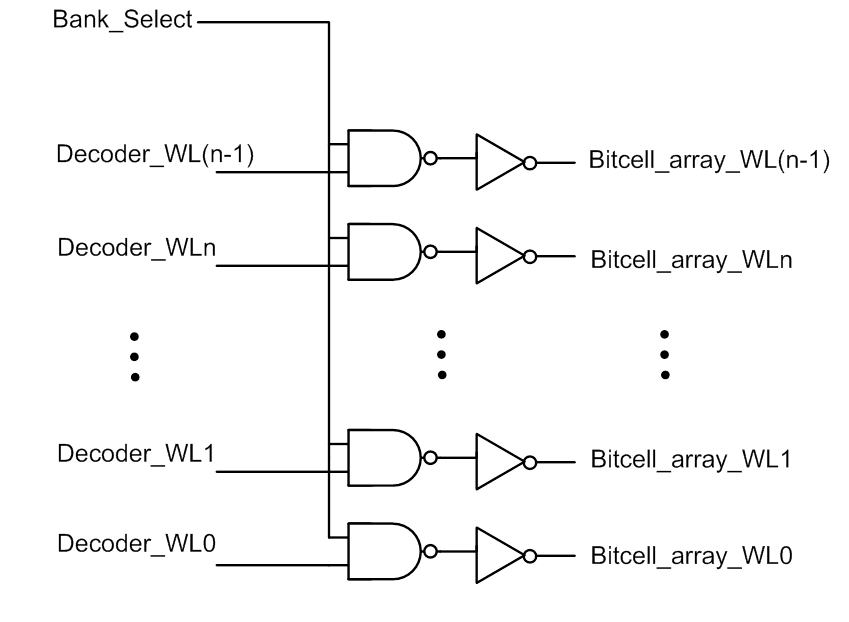
\includegraphics[scale=.8]{./figs/wordline_driver.pdf}
\caption{Diagram of word line driver.}
\label{fig:wordline_driver}
\end{figure}


\subsection{Column Mux}

The column mux takes the column address bits from the address bus
selects the appropriate bitlines for the word that is to be read from
or written to.  It takes n-bits from the address bus and can select
$2^n$ bitlines. The column mux is used for both the read and write
operations; it connects the bitline of the memory array to both the
sense ampflifier and the write driver.

OpenRAM provides several options for column mux, but the default
is a single-level column mux which is sized for optimal speed.

\subsubsection{Tree\_Decoding Column Mux}
\label{sec:tree_decoding_column_mux}

The schematic for a 4-1 tree
multiplexer is shown in Figure~\ref{fig:colmux}.

\begin{figure}[h!]
\centering
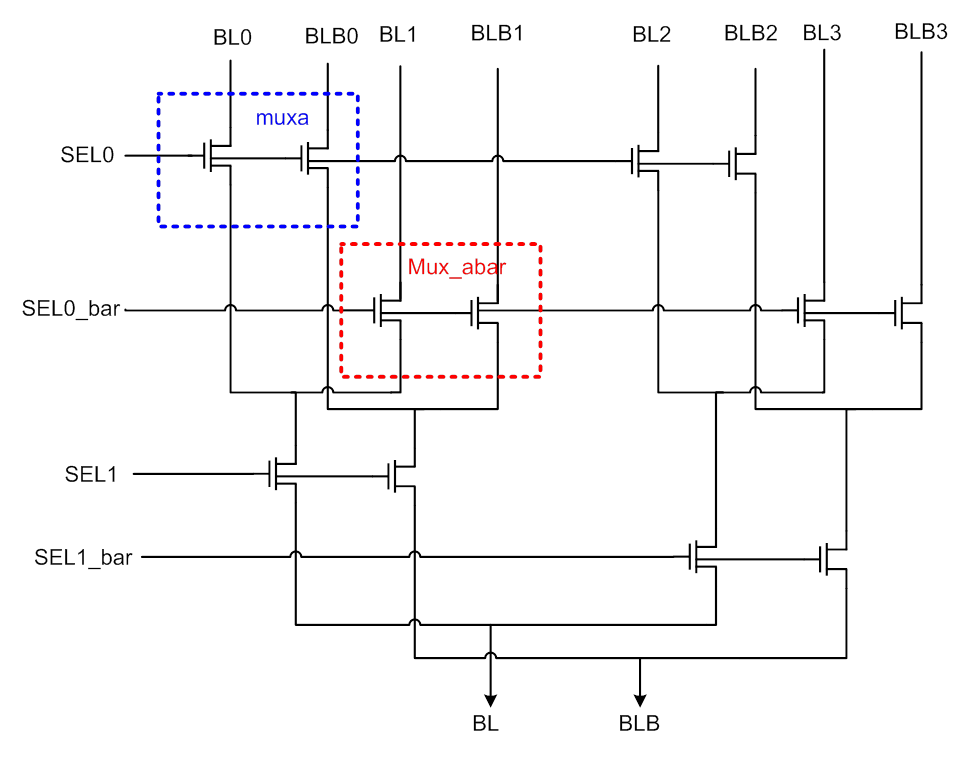
\includegraphics[scale=.9]{./figs/tree_column_mux_schem.pdf}
\caption{Schematic of 4-1 tree column mux that passes both of the bitlines.}
\label{fig:colmux}
\end{figure}

\fixme{Shading/opacity is different on different platforms. Make this a box in the image. It doesn't work on OSX.}

This tree mux selects pairs of bitlines (both BL and BL\_B) as inputs
and outputs.  This 4-1 tree mux illustrates the process of choosing
the correct bitlines if there are 4 words per row in the memory array.
Each bitline pair represents a single bit from each word.  A binary
reduction pattern, shown in Table~\ref{table:colmux}, is used to
select the appropriate bitlines.  As the number of words per row in
the memory array increases, the depth of the column mux grows.  The
depth of the column mux is equal to the number of bits in the column
address bus.  The 4-1 tree mux has a depth of 2.  In level 1, the
least significant bit from the column address bus selects either the
first and second words or the third and fourth words.  In level 2, the
most signifant column address bit selects one of the words passed down
from the previous level.  Relative to other column mux designs, the
tree mus uses significantly less devices.  But, this type of design
can provide poor performance if a large decoder with many levels are
needed.  The delay of of a tree mux quadratically increases with each
level.  Due to this fact, other types of column
decoders should be considered for larger arrays.

\begin{table}[h!] 
  \begin{center}
    \begin{tabular}{| c | c | c | c |}
    \hline
    Selected BL & Inp1 & Inp2 & Binary\\ \hline
    BL0 & SEL0\_bar & SEL1\_bar & 00\\ \hline
    BL1 & SEL0 & SEL1\_bar & 01\\ \hline
    BL2 & SEL0\_bar & SEL1 & 10\\ \hline
    BL3 & SEL0 & SEL1 & 11\\
    \hline
    \end{tabular}
  \end{center}
  \caption{Binary reduction pattern for 4-1 tree column mux.}
  \label{table:colmux}
\end{table} 

In OpenRAM, the tree column mux is a dynamically generated design.  The
\verb|tree_mux_array| is made up of two dynamically generated cells: \verb|muxa|
and \verb|mux_abar|.  The only diffference between these cells is that input
select signal is either hooked up to the \textbf{SEL} or
\textbf{SEL\_bar} signals (see highlighted boxes in
Figure~\ref{fig:colmux}).  These cells are initialized the the
\verb|column_muxa| and \verb|column_muxabar| classes in \verb|columm_mux.py|.  Instances
of \verb|ptx| PMOS transistors are added to the design and the necessary
routing is performed using the \verb|add_rect()| function. A horizontal rail
is added in metal2 for both the SEL and Sel\_bar signals.  Underneath
those input rails, horizontal straps are added.  These straps are used
to connect the BL and BL\_B outputs from \verb|muxa| to the BL and BL\_B
outputs of \verb|mux_abar|.  Vertical conenctors in metal3 are added at the
bottom of the cell so that connections can be made down to the sense
amp.  Vertical connectors are also added in metal1 so that the cells
can connect down to other mux cells when the depth of the tree mux is
more than one level.

The \verb|tree_mux_array| class is used to generate the tree mux.
Instances of both the \verb|muxa| and \verb|mux_abar| cells are instantiated and
are tiled row by row.  The offset of the cell in a row is determined
by the depth of that row in the tree mux.  The pattern used to
determine the offset of the mux cells is
$muxa.width*(i)*(2*row\_depth)$ where is the column number.  As the
depth increases, the mux cells become further apart.  A separate
``for'' loop is invoked if the $depth>1$, which extends the
power/ground and select rails across the entire width of the array.
Similarly, if the $depth>1$, spice net names are created for the
intermediate connection made at the various levels.  This is necessary
to ensure that a correct spice netlist is generated and that the
input/output pins of the column mux match the pins in the modules that
it is connected to.


\subsubsection{Single\_Level Column Mux}
\label{sec:single_level_column_mux}

The optimal design for column mux uses a single NMOS device, driven by the input address or decoded input addresses.
Figure~\ref{fig:2t1_single_level_column_mux} shows the schematic of a 2:1 single-level column mux. In this column mux one bit 
of address and its complementry drive the pass transistors. Selected transistors will  
connect their corresponding bitlines ( 1 set of column out of 2 set of columns) to sense-amp and write-driver circuitry for read or write operation. 
Figure~\ref{fig:4t1_single_level_column_mux} shows the schematic of a 4:1 single-level column mux. In this column mux, 2 input 
address are decoded using a 2:4 decoder ( 2:4 decoder is explain in section~\ref{sec:hierdecoder}). 2:4 decoder provides a one-hot set of outputs, so only one set of columns 
will be selected and connected to sense-amp and write-driver
( in figure~\ref{fig:4t1_single_level_column_mux} one set of column out of four sets of column is selected).

In OpenRAM, the \verb|single-level_mux_array| is a dynamically generated design and 
it is made up of dynamically generated cell (\verb|single-level_mux|).
\verb|single-level_mux| uses the parameterized transistor class \verb|ptx| to generate two NMOS transistors 
which will connect the BL and BLB of selected columns to sense-amp and write-driver. Horizontal rails are added for $sel$ signals. Vertical   
straps connect the BL and BLB of bitcell\_array to BL and BLB of single-level column mux and also BL-out and BLB-out of single-level 
column mux to BL and BLB of sense-amp and write-driver.


\begin{figure}[h!]
\centering
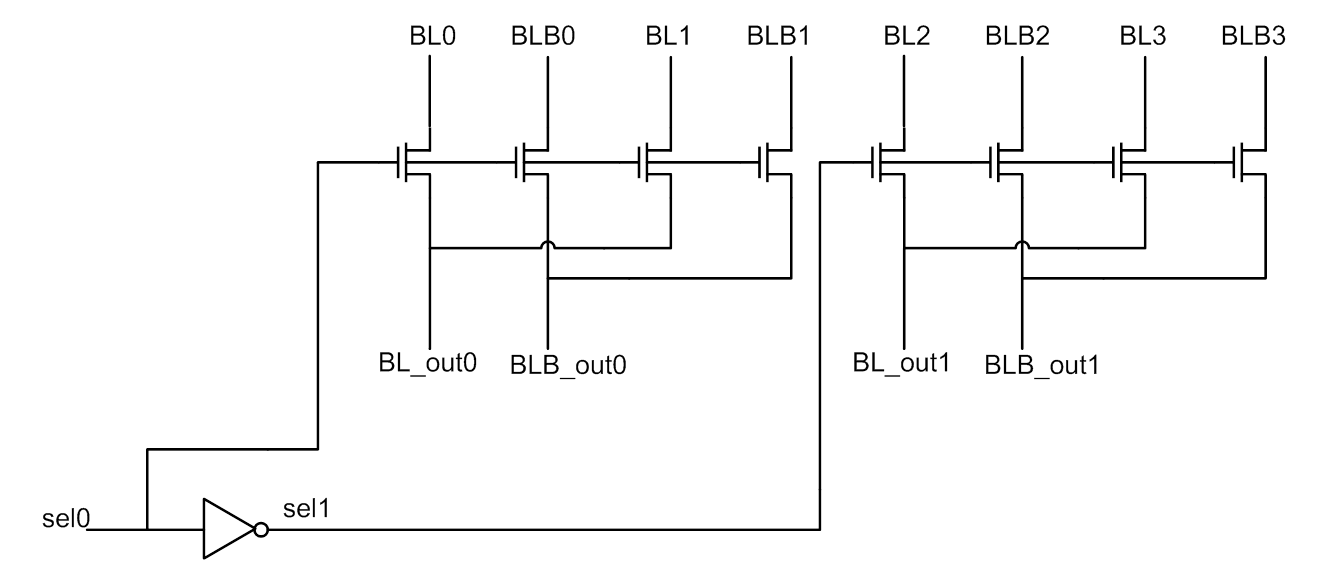
\includegraphics[scale=.7]{./figs/2t1_single_level_column_mux.pdf}
\caption{Schematic of a 2:1 single level column mux.}
\label{fig:2t1_single_level_column_mux}
\end{figure}



\begin{figure}[h!]
\centering
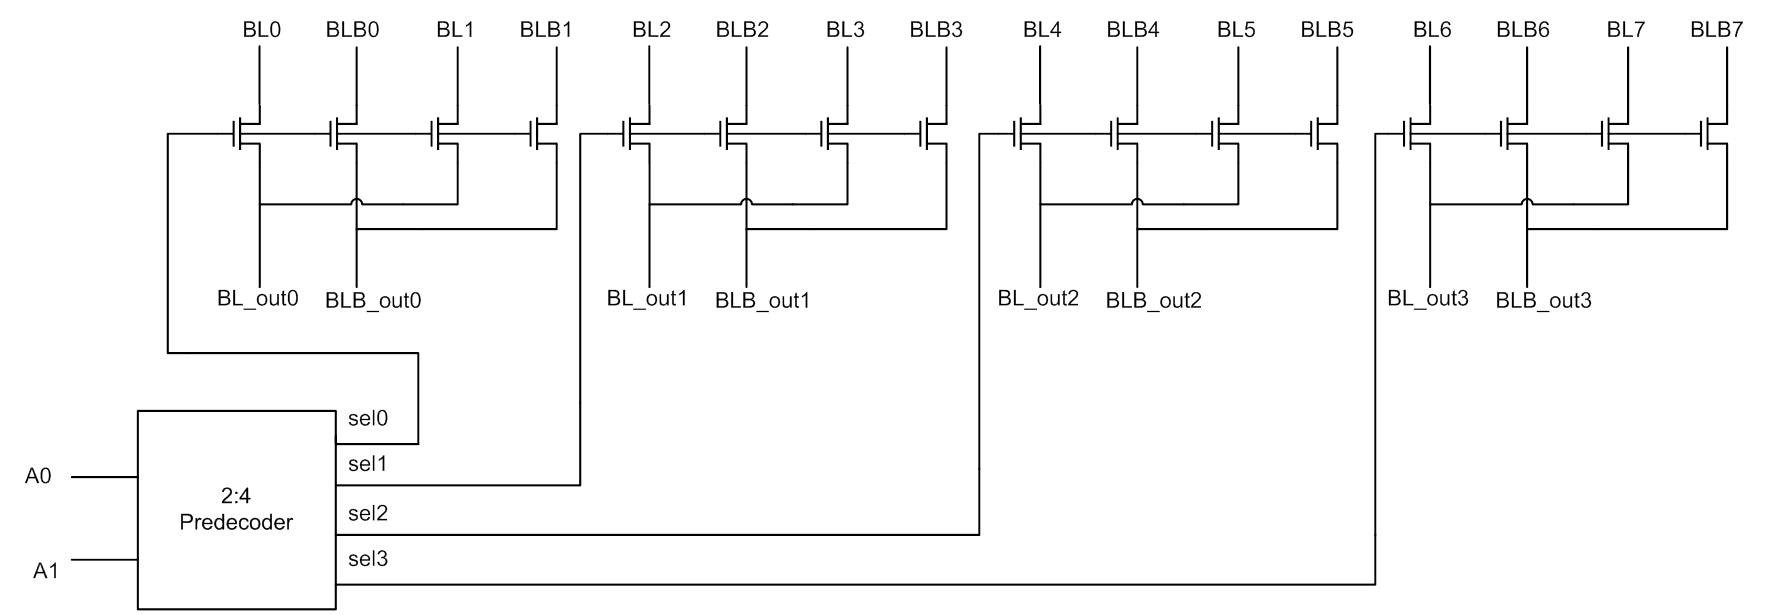
\includegraphics[scale=.6]{./figs/4t1_single_level_column_mux.pdf}
\caption{Schematic of a 4:1 single level column mux.}
\label{fig:4t1_single_level_column_mux}
\end{figure}


\subsection{Sense Amplifier}
\label{sec:senseamp}
The sense amplifier is used to sense the difference between the
bitline and bitline bar while a read operation is performed.  The
sense amp is necessary to recover the signals from the bitlines
because they do not experience full voltage swing.  As the size of the
memory array grows, the load of the bitlines increases and the voltage
swing is limited by the small memory cell driving this large load.  A
differential sense amplifier is used to``sense'' the small voltage
difference between the bitlines.

\begin{figure}[h!]
\centering
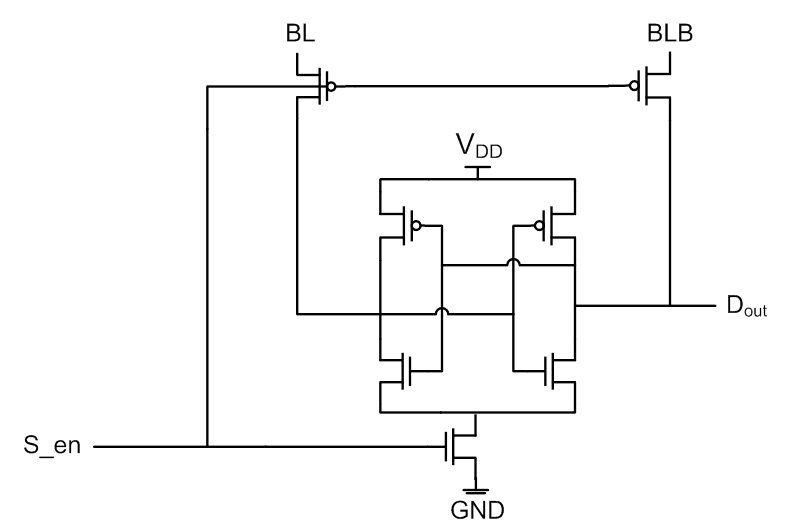
\includegraphics[scale=.8]{./figs/sense_amp_schem.pdf}
\caption{Schematic of a single sense amplifier cell.}
\label{fig:sense_amp}
\end{figure}

The schematic for the sense amp is shown in
Figure~\ref{fig:sense_amp}.  The sense amplifier is enable by the SCLK
signal, which initiates the read operation.  Before the sense
amplifier is enable, the bitlines are precharged to Vdd by the
precharge unit.  When the sense amp is enabled, one of the bitlines
experiences a voltage drop based on the value stored in the memory
cell.  If a zero is stored, the bitline voltage drops.  If a one is
stored, the bitline bar voltage drops.  The output signal is then
taken to a true logic level and latched for output to the data bus.

In OpenRAM, the sense amplifier is a libray cell.  The associated
layout and spice netlist can be found in the \verb|gds_lib| and \verb|sp_lib| in
the FreePDK45 directory.  The \verb|sense_amp| class in \verb|sense_amp.py|
instantiates a single instance of the sense amp library cell.  The
\verb|sense_amp_array| class handles the tiling of the sense amps cells.
One sense amp cell is needed per data bit and the sense amp cells need
to be appropriately spaced so that they can hook up to the column mux
bitline pairs.  The spacing is determined based on the number of words
per row in the memory array.  Instances are added and then Vdd, Gnd
and SCLK rails that span the entire width of the array are drawn using
the add\_rect() function.

We chose to leave the sense amp as a libray cell so that custom
amplifier designs could be swapped into the memory as needed.  The two
major things that need to be considered while designing the sense
amplifier cell are the size of the cell and the bitline/input pitches.
Optimally, the cell should be no larger than the 6T cell so that it
abuts to the column mux and no extra routing or space is needed.
Also, the bitline inputs of the sense amp need to line up with the
outputs of the write driver.  In the current version of OpenRAM, the
write driver is situated under the sense amp, which had bitlines
spaning the entire height of the cell.  In this case, the sense
amplifier is disabled during a write operation but the bitlines still
connect the write driver to the column mux without any extra routing.


\subsection{Write Driver}
\label{sec:writedriver}
The write driver is used to drive the input signal into the memory
cell during a write operation.  It can be seen in
Figure~\ref{fig:write_driver} that the write driver consists of two
tristate buffers, one inverting and one non-inverting.  It takes in a
data bit, from the data bus, and outputs that value on the bitline,
and its complement on bitline bar.  The bitlines need to be
complements so that the data value can be correctly stored in the 6T
cell. Both tristates are enabled by the EN signal.

\begin{figure}[h!]
\centering
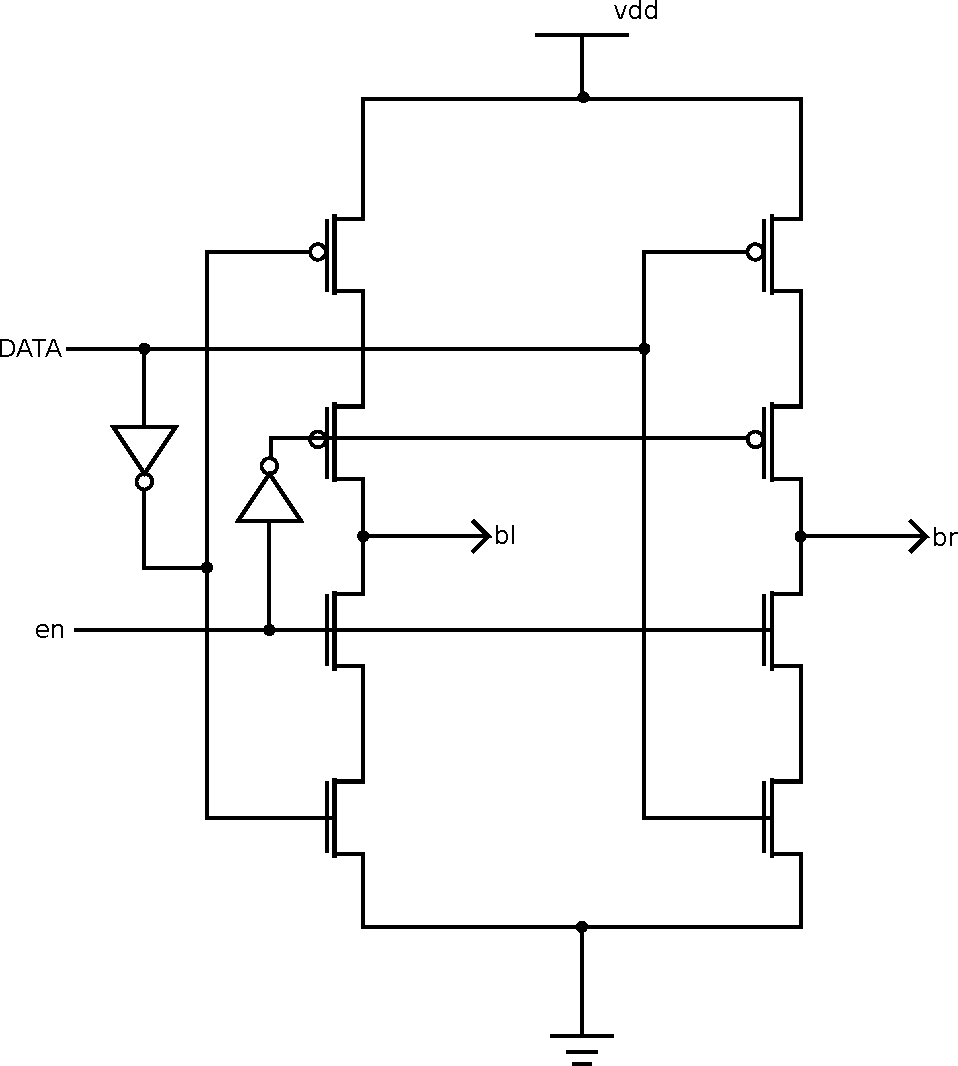
\includegraphics[scale=.8]{./figs/write_driver_schem.pdf}
\caption{Schematic of a write driver cell, which consists of 2 tristates (non-inverting and inverting) to drive the bitlines.}
\label{fig:write_driver}
\end{figure}

Currently, in OpenRAM, the write driver is a library cell.  The
associated layout and spice netlist can be found in the \verb|gds_lib| and
\verb|sp_lib| in the FreePDK45 directory.  Similar to the \verb|sense_amp_array|,
the \verb|write_driver_array| class tiles the write driver cells.  One
driver cell is needed per data bit and Vdd, Gnd, and EN signals must
be extended to span the entire width of the cell. It is not optimal to
have the write driver as a library cell because the driver needs to be
sized based on the capacitance of the bitlines.  A large memory array
needs a stronger driver to drive the data values into the memory
cells.  We are working on creating a parameterized tristate class,
which will dynamically generate write driver cells of different
sizes/strengths.

\subsection{Flip-Flop Array}

In a synchronous SRAM it is necessary to synchronize the inputs and
outputs with a clock signal by using flip-flops.  In FreePDK45 we
provide a library cell for a simple master-slave flip-flop, see
schematic in Figure~\ref{fig:ms_flop}.  In our library cell we provide
both Q and Q\_bar as outputs of the flop because inverted signals are
used in various modules.  The \verb|ms_flop| class in \verb|ms_flop.py|
instatitates a single master-slave flop, and the \verb|ms_flop_array| class
generates an array of flip-flops.  Arrays of flops are necessary for
the data bus (an array for both the inputs and outputs) as well as the
address bus (an array for row and column inputs).  The \verb|ms_flop_array|
takes the number of flops and the type of array as inputs.  Currently,
the type of the array must be either ``data\_in'', ``data\_out'',
``addr\_row'', or ``addr\_col'' verbatim.  The array type input is
used to look up that associated pin names for each of the flop arrays.
This was implemented very quickly and should be improved in the near
future...

\begin{figure}[h!]
\centering
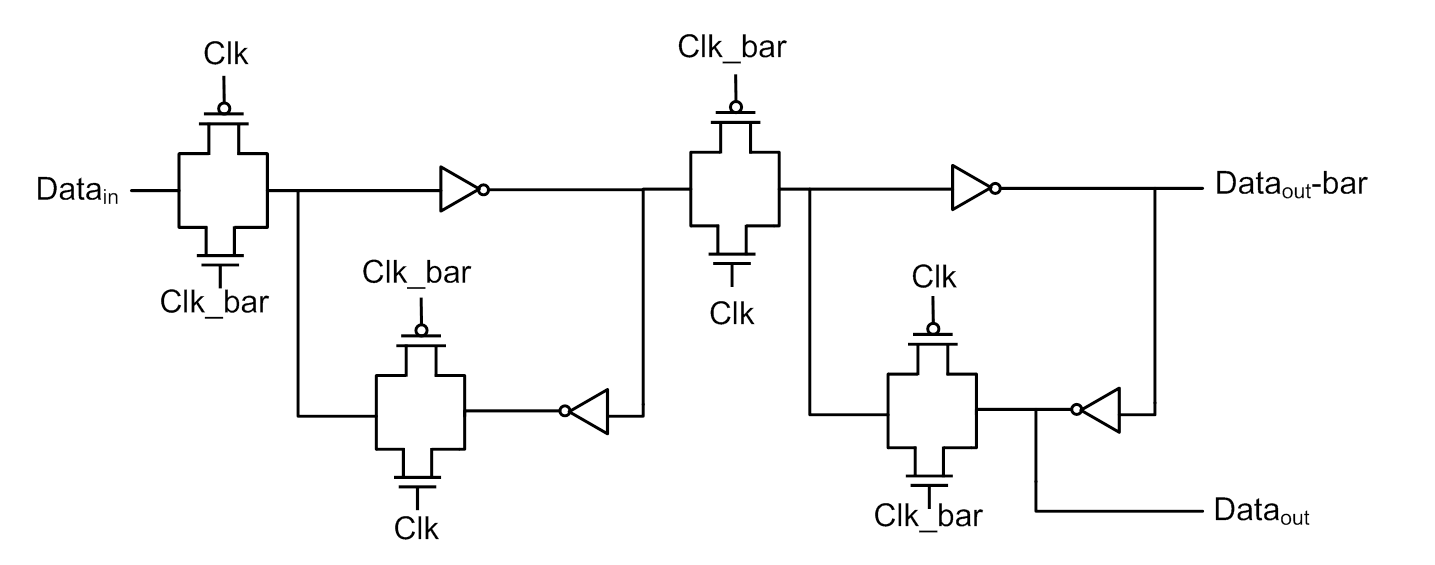
\includegraphics[scale=.7]{./figs/ms_flop_schem.pdf}
\caption{Schematic of a master-slave flip-flop provided in FreePDK45 library}
\label{fig:ms_flop}
\end{figure}

\subsection{Control Logic}

The details of the control logic architecture are outlined in
Section~\ref{sec:control}.  The control logic module,
\verb|control_logic.py|, instantiates a \verb|control_logic| class that arranges
all of the flip-flops and logic associated with the control signals
into a single module. Flip-flops are instantiated for each control
signal input and library NAND and NOR gates are used for the logic.  A
delay chain, of variable length, is also generted using parameterized
inverters.  The associated layouts and spice netlists can be found in
the \verb|gds_lib| and \verb|sp_lib| in the FreePDK45 directory.

\section{Bank and SRAM}
\label{sec:bank}

The overall memory architecture is shown in figure~\ref{fig:bank}.
As shown in this figure one Bank contains different modules including 
precharge-array which is positioned above the bitcell-array, 
column-mux-array which is located below the bitcell-array, 
sense-amp-array, write-driver-array, data-in-ms-flop-array 
to synchronize the input data with negative edge of the clock, 
tri-gata-array to share the bidirectional data-bus between input 
and output data, hierarchical decoder which is placed on the right side 
of the bitcell-array (predecoder + decoder), wordline-driver which drives 
the wordlines horizontally across the bitcell-array and address-ms-flops 
to synchronize the input address with positive edge of the clock. 

In bitcell-array each memory cell is mirrored vertically and horizontally inorder to share VDD and GND rails with adjacent cells and form the array. 
Data-bus is connected to tri-gate, address-bus is connected to address-ms-flops and bank-select 
signal will enable the bank when it goes high. To complete the SRAM design, bank is connected to control-logic as shown in figure~\ref{fig:bank}. 
Control-logic controls the timing 
of modules inside the bank. CSb, OEb, Web and clk are inputs to the control logic and output of 
control logic will ANDed with bank-select signal and send to the corresponding modules.


\begin{figure}[h!]
\centering
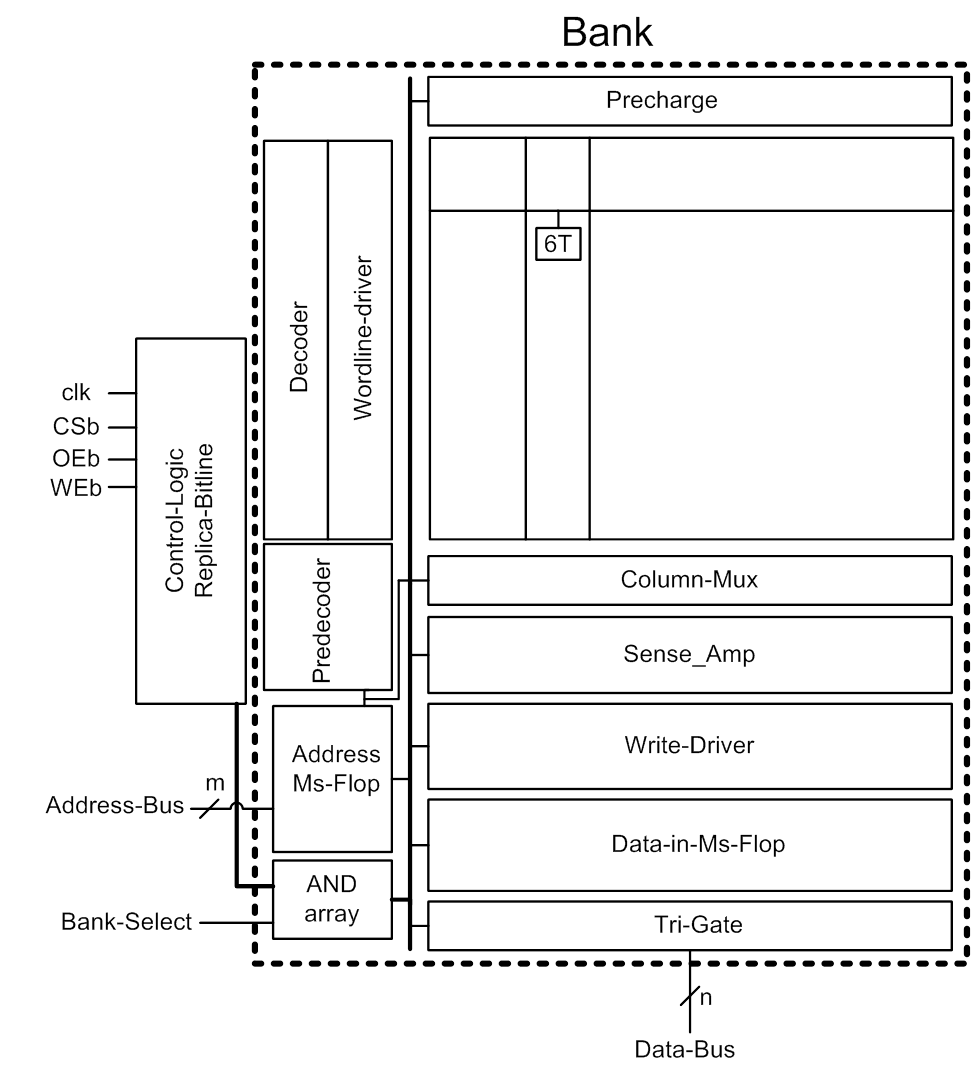
\includegraphics[scale=1]{./figs/bank.pdf}
\caption{Overal bank and SRAM architecture.}
\label{fig:bank}
\end{figure}


In order to reduce the delay and power, divided wordline strategy have been used in this compiler. Part of the address bits 
are used to define the global wordline (bank-select) and rest of address bits are connected to hierarchical 
decoder inside each bank to generate local wordlines that actually drive the bitcell access transistors. 

As shown in figure~\ref{fig:bank2} SRAM is divided to two banks which share data-bus, address-bus, control-bus and control-logic. 
In this case one bit of address (most significant bit) goes to an ms-flop and outputs of ms-flop (address-out and address-out-bar) 
are connected to banks as bank-select signals. Control logic is shared between two banks and based on which bank is selected, 
control signals will activate modules inside the selected bank. In this architecture, the total cell capacitance is reduced by up 
to a factor of two. Therefore the power will be reduced greatly and the delay among the wordlines is also reduced.

\begin{figure}[h!]
\centering
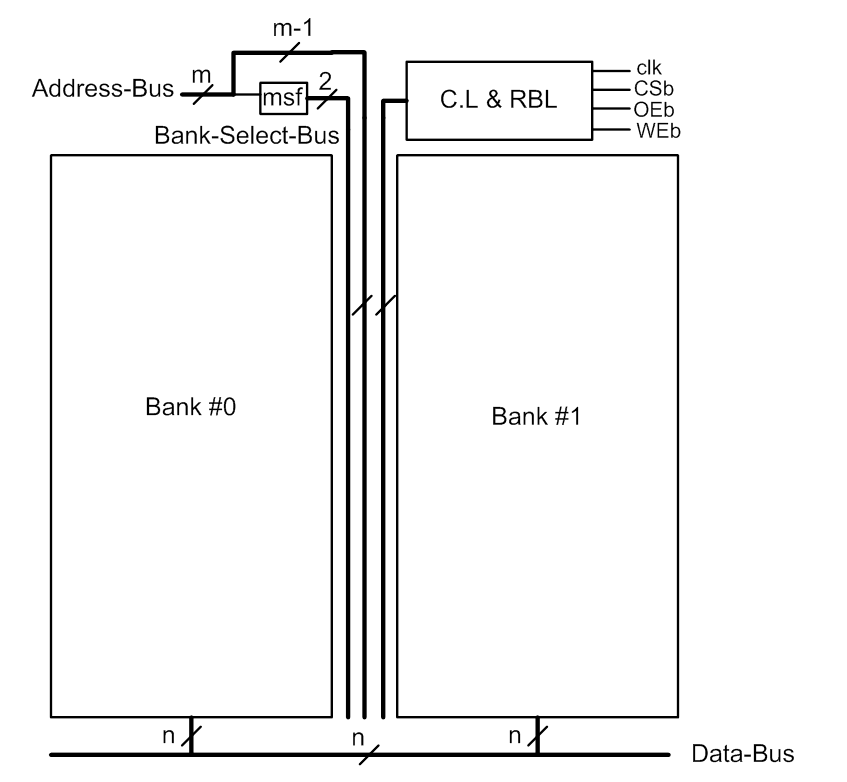
\includegraphics[scale=.9]{./figs/bank2.pdf}
\caption{SRAM is divided to two banks which share the control-logic.}
\label{fig:bank2}
\end{figure}

In figure~\ref{fig:bank4}, four banks are connected together. In this case a 2:4 decoder is added to select one of the banks using two 
most significant bits of input address. Control signals are connected to all banks but will turn on only the selected bank.


\begin{figure}[h!]
\centering
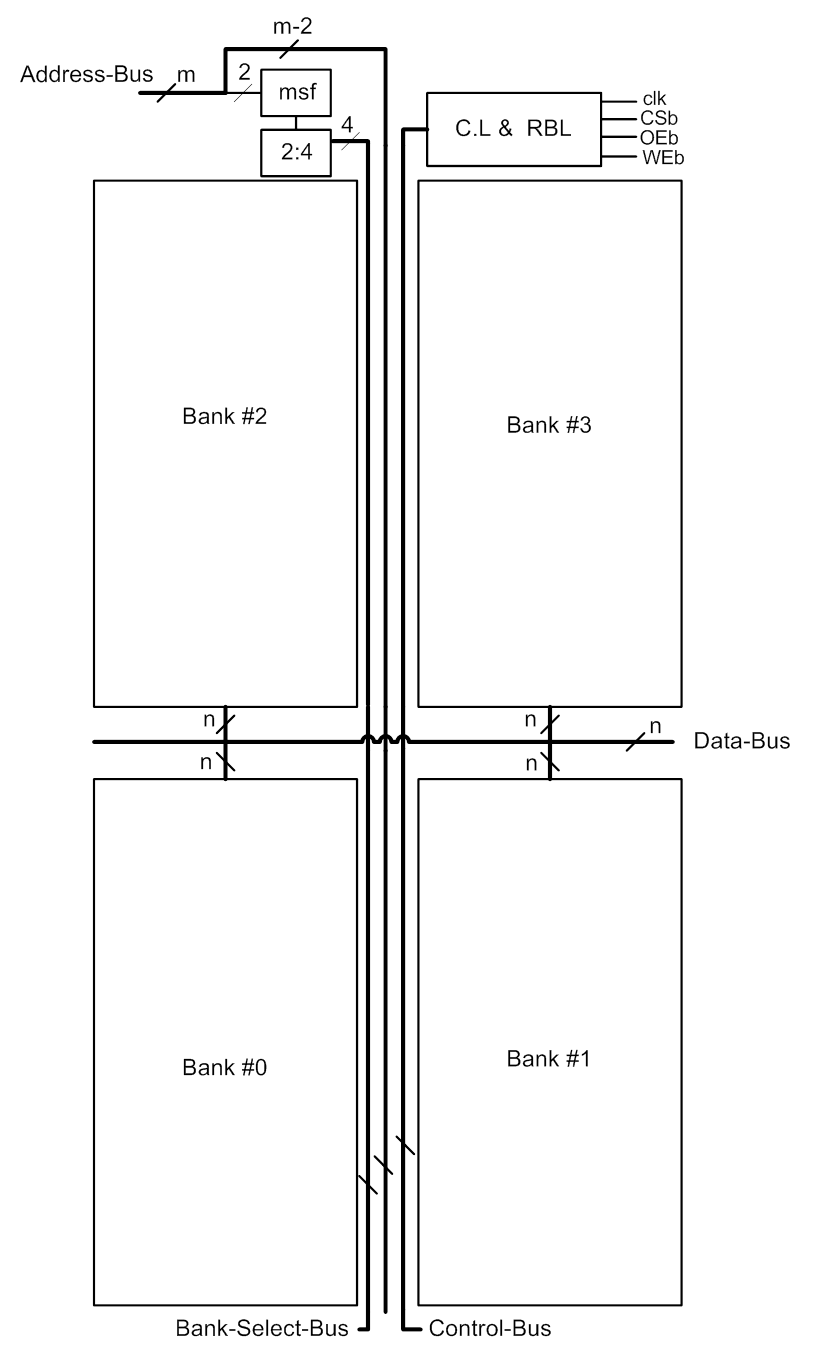
\includegraphics[scale=.9]{./figs/bank4.pdf}
\caption{SRAM is divided to 4 banks wich are controlled by the control-logic and a 2:4 decoder.}
\label{fig:bank4}
\end{figure}


